\chapter{差动放大电路的设计与仿真}%
\label{cha:差动放大电路的设计与仿真}

\section{实验目的}%
\label{sec:\arabic{chapter}实验目的}

\begin{enumerate}
	\item 设计一个带恒流源的差动放大电路,要求空载时的$ A_\mathrm{VD} $大于20;
	\item 给电路输入\SI{10}{\mV}的直流差模小信号,分别测试电路的双端输出的差模增益$ A_\mathrm{VD} $、单端输出的差模增益$ A_\mathrm{VD1} $;
	\item 给电路输入\SI{1}{\V}的直流共模信号,分别测试双端输出的共模增益$ A_\mathrm{VC} $以及单端输出的共模增益$ A_\mathrm{VC1} $值;
	\item 测量差分放大电路的传输特性曲线。
\end{enumerate}

\section{实验要求}%
\label{sec:\arabic{chapter}实验要求}

\begin{Exercise}
	给出自行设计的差分放大电路原理图,测量其空载时的差模增益。
\end{Exercise}

\begin{Answer}
	差分放大电路原理图见图\ref{fig:差动放大电路原理图},空载时的差模增益见表\ref{tab:差分放大电路参数}。
\end{Answer}

\begin{Exercise}
	给出测量双端输出和单端输出差模增益的电路,求出差模增益的值,并说明单端输出时从$ Q_1 $管输出和从$ Q_2 $管输出的不同。
\end{Exercise}

\begin{Answer}
	双端输出和单端输出电路图见\ref{fig:差动放大电路原理图},差模增益见表\ref{tab:差分放大电路参数},不同是符号相反。
\end{Answer}

\begin{Exercise}
	给出测量双端输出和单端输出共模增益的电路。求出共模增益,并计算共模抑制比。
\end{Exercise}

\begin{Answer}
	测量双端输出和单端输出共模增益的电路图见图\ref{fig:输入共模信号}。共模增益、共模抑制比见表\ref{tab:差分放大电路参数}。
\end{Answer}

\begin{Exercise}
	给出电压传输特性曲线,并对曲线进行必要的说明。
\end{Exercise}

\begin{Answer}
	电压传输特性曲线见图\ref{fig:差动放大电路直流传输特性},说明见章节\ref{sub:\arabic{chapter}仿真结果}。
\end{Answer}

\begin{Exercise}
	分析实验结果。
\end{Exercise}

\begin{Answer}
	分析见章节\ref{sec:\arabic{chapter}实验小结}。
\end{Answer}

\section{实验步骤}%
\label{sec:\arabic{chapter}实验步骤}

\subsection{设计电路}%
\label{sub:\arabic{chapter}设计电路}

\begin{figure}[H]
	\centering
	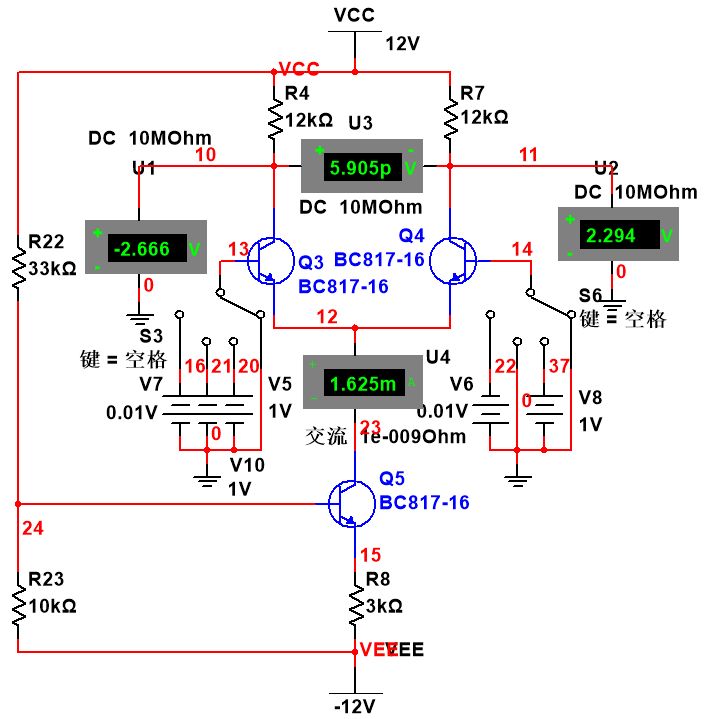
\includegraphics[width=0.8\linewidth]{2/V0.png}
	\caption{差动放大电路原理图}
	\label{fig:差动放大电路原理图}
\end{figure}

如图\ref{fig:差动放大电路原理图}所示,将开关拨到不同位置可以输入不同的信号。输入差模信号见图\ref{fig:输入差模信号},输入共模信号见图\ref{fig:输入共模信号}。

\begin{figure}[H]
	\centering
	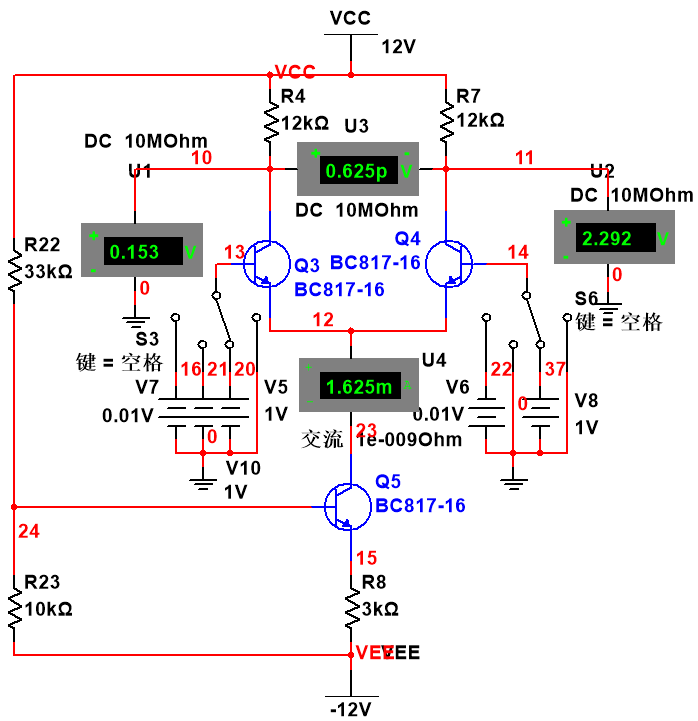
\includegraphics[width=0.8\linewidth]{2/Vc.png}
	\caption{输入差模信号}
	\label{fig:输入差模信号}
\end{figure}

\begin{figure}[H]
	\centering
	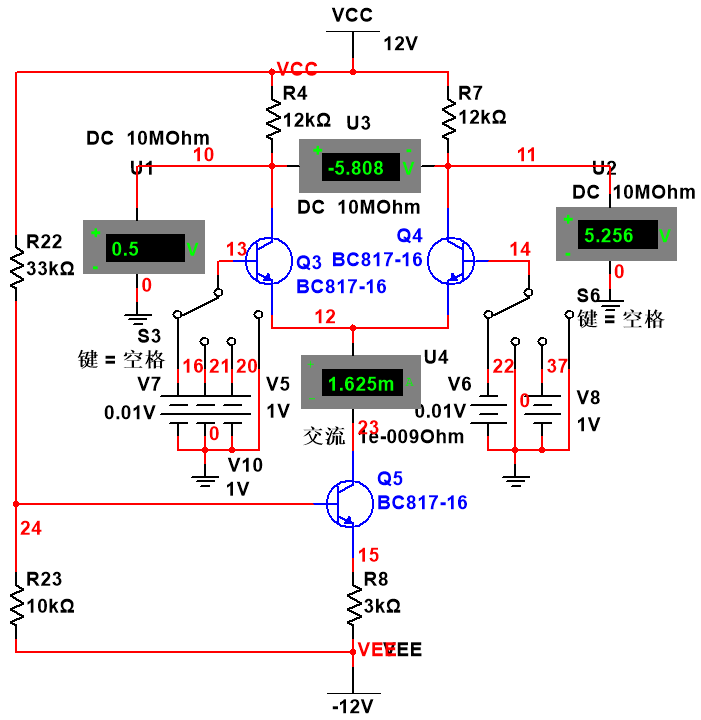
\includegraphics[width=0.8\linewidth]{2/Vd.png}
	\caption{输入共模信号}
	\label{fig:输入共模信号}
\end{figure}

\subsection{指标计算}%
\label{sub:\arabic{chapter}指标计算}

\begin{table}[H]
	\centering
	\caption{差分放大电路参数}
	\label{tab:差分放大电路参数}
	\csvautobooktabular{tab/2/2-1.csv}
\end{table}

\subsection{仿真结果}%
\label{sub:\arabic{chapter}仿真结果}

\begin{figure}[H]
	\centering
	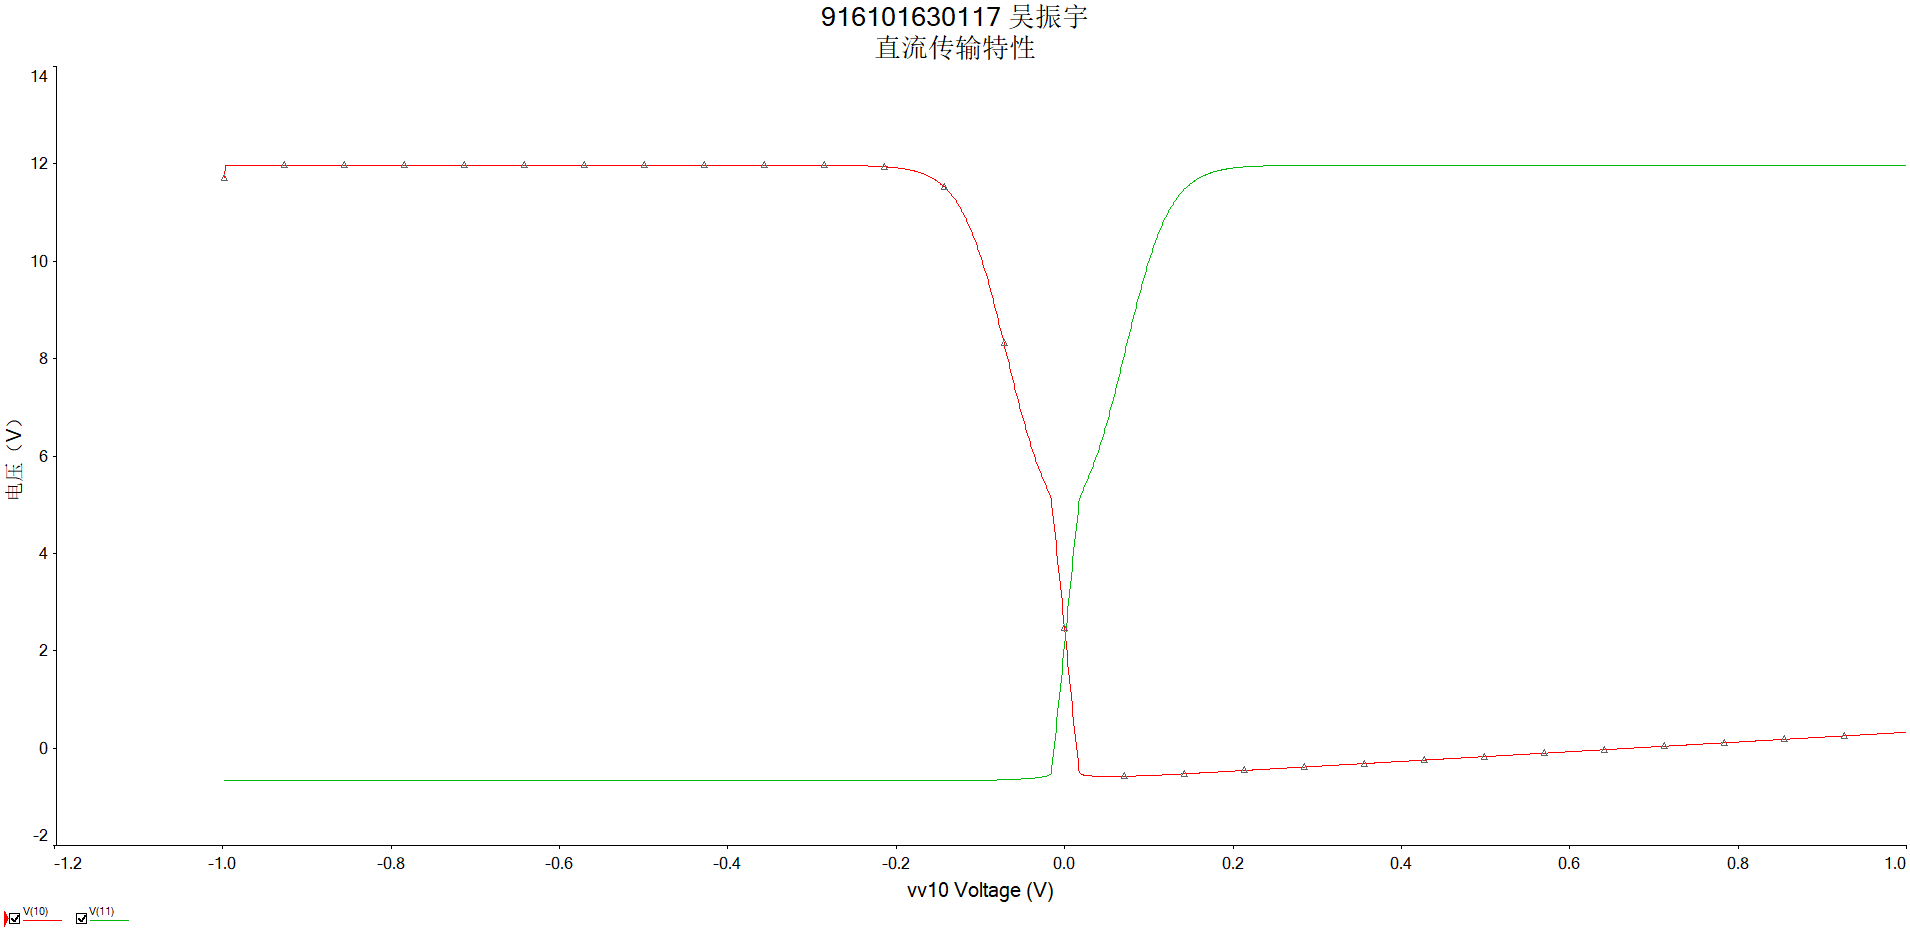
\includegraphics[width=0.8\linewidth]{2/diff.png}
	\caption{差动放大电路直流传输特性}
	\label{fig:差动放大电路直流传输特性}
\end{figure}

差动放大电路直流传输特性曲线见图\ref{fig:差动放大电路直流传输特性},该曲线的对称验证了从$ Q_1 $管输出和从$ Q_2 $管输出的不同是符号相反。

\subsection{误差分析}%
\label{sub:\arabic{chapter}误差分析}

误差分析见表\ref{tab:差动放大电路误差分析},可以看出仿真结果与理论推导相差较小。

\begin{table}[H]
	\centering
	\caption{差动放大电路误差分析}
	\label{tab:差动放大电路误差分析}
	\csvautobooktabular{tab/2/2-2.csv}
\end{table}

\section{实验小结}%
\label{sec:\arabic{chapter}实验小结}

通过此次实验可以看出,差分放大电路对共模信号有着强烈的抑制效果,因为其有这样的特性,所以在现实生活中应用广泛。

